\graphicspath{{../images/ch4/}}	% Image directory


\chapter{Resistive pulse studies of aspherical mesoparticles}

	

	\section{Background \& Theory}
		In the introduction of this dissertation we introduced and explained the theory behind resistive pulse sensing, a particle characterization technique that works by monitoring the change in conductance of a nanopore as small particles pass through it. Probably the most important application of RP sensing is in measuring the sizes of particles. An analytic model was devised by DeBlois \emph{et al.} to relate the size of a particle to its resistive pulse amplitude. The solution is essentially an electrostatics boundary-value problem: given an insulating particle inside a pore and a known externally applied voltage, calculate the electric field distribution inside the pore, and from the electric field distribution calculate the pore's expected resistance with the particle inside it. When this calculation is performed for spherical particles travelling along the axis of long cylindrical pores, the change in resistance or current is found to be
		
		\begin{equation}\label{eq:dI}
			\frac{\Delta R}{R_{0}}=\frac{\Delta I}{I_{p}}=\frac{4\rho D^{3}}{\pi d^{4}}\left[1-0.8\left(\frac{d}{D}\right)^{3}\right].
		\end{equation}
		
		Equation \ref{eq:dI} is useful for relating the change in current---or resistance---to the diameter of spherical particles. However, it is very often the case that particles of interest are not spherical. For instance, many biomolecules such as viruses and proteins are poorly approximated as spheres, and are more rod-like in shape. In this case, the resistive pulse amplitude of on-axis translocations through a cylindrical pore is given by 
		
		\begin{equation}{\label{eq:dIellipsoid}
			\frac{\Delta R}{R_{0}}=\left[f_{\perp}+\left(f_{\parallel}-f_{\perp}\cos^{2}\alpha]right]\frac{v}{V},
		\end{equation}

		where $f_{\perp}$ and $f_{\parallel}$ are so called `shape-factors', that depend on the particle's major and minor axis lengths, $\alpha$ is the orientation of the particle with $\alpha=0$ being axially aligned, and $v$ and $V$ are the volume of the particle and of the pore, respectively. Figure \ref{fig:dIellipsoid} shows a plot of the relative $\Delta I/I_{p}$ for various ellipsoids of the same volume but different axial lengths.
		
		\begin{figure}
			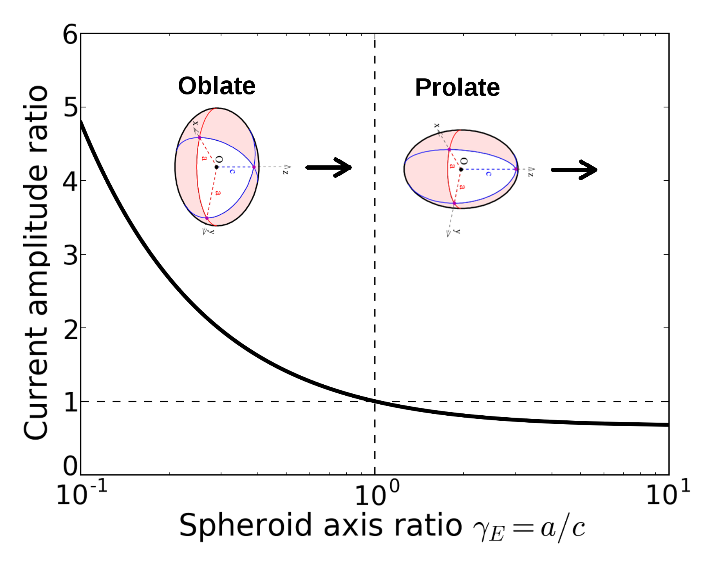
\includegraphics[width=0.5\textwidth]{dIellipsoid}
			\caption{adsf}
			\label{fig:dIellipsoid}
		\end{figure}

		
		
		
		
		
		
		While equation \ref{eq:dIellipsoid} is useful for determining the volume of spheroidal particles from their resistive pulse amplitudes, it would be useful to devise a method for measuring the length of particles in addition to measuring their volumes as an additional physical marker for their identification in a sample.
		
		Consider a pore with a rough, non-uniform interior. Due to the irregular interior, the channel cross sections will have a range of resistance values; for instance, a large cavity in the channel will have a smaller resistance than a more narrow constriction. If a very small particle travels through the pore, its resistive pulse time-series is determined by the interior topology of the pore. For instance, when it happens to occupy a narrower region of the pore, the resistance in tha tregion is larger relative to the rest of the pore, and therefore the particle  will also block a relatively larger portion of the current. In this way, the particle is able to resolve the interior features of the pore. In such cases, the instantaneous resistive pulse amplitude is given by 
		
		\begin{equation}\label{eq:dIlocal}
			\Delta R=R_{p}-R_{0}=\frac{4\rho d^{3}}{\pi D^{4}}\left[1-0.8\left(\frac{d}{D}\right)^{3}\right]^{-1}.
		\end{equation}

		
		Oppositely, if we consider a pore whose length extends along a significant amount of the pore's axis, it may be occupying several such regions at a time. Instead of a single particle, we may consider the particle to be composed of many smaller segments of particles in series, and therefore the resistsance values of each segment are additive. Therefore, the signals of longer particles can be seen as the convolution of the signal of an infinitesimally small particle over the long particle's length. 
		
		This fact can be used to devise an experiment that can measure the length of long particles. First, we drive a suspension of small `tracer' spheres through a pore with rough interior, whose diameter is smaller than the characteristic length of the irregularities in the pore. These particles will `map' the interior geometry of the pore as explained above, with resistive pulse shape given by equation \ref{eq:dIlocal}. Then, we repeat the experiment with long particles for which we wish to know the length. Then we perform a convolution or moving average of the signals of the tracer particles for a variety of lengths; finally, a similarity measure is calculated between every pair of convoluted-raw signals for the tracer particle and the long particle, and the length with the greatest similarity measure is chosen as the correct length of the particle. 
		
	\section{Experiment}
	    
		\begin{figure}
			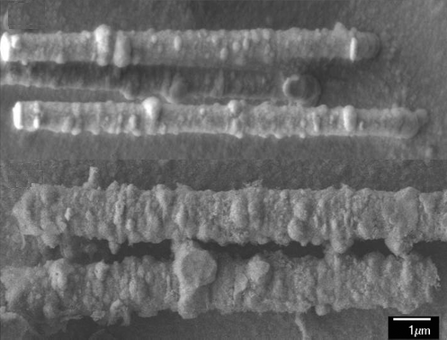
\includegraphics[width=0.5\textwidth]{PET}
			\caption{\textbf{Scanning electron microscope images of metal replica of track-etched PET pores.} The pores were filled with metal and the polymer was completely etched a way, leaving a metal structure that is the inverse of the pore. The metal was imaged in a scanning electron microscope. The images reveal the irregular shapes of the PET pore surfaces.}

		\end{figure}
		
		\begin{figure}
			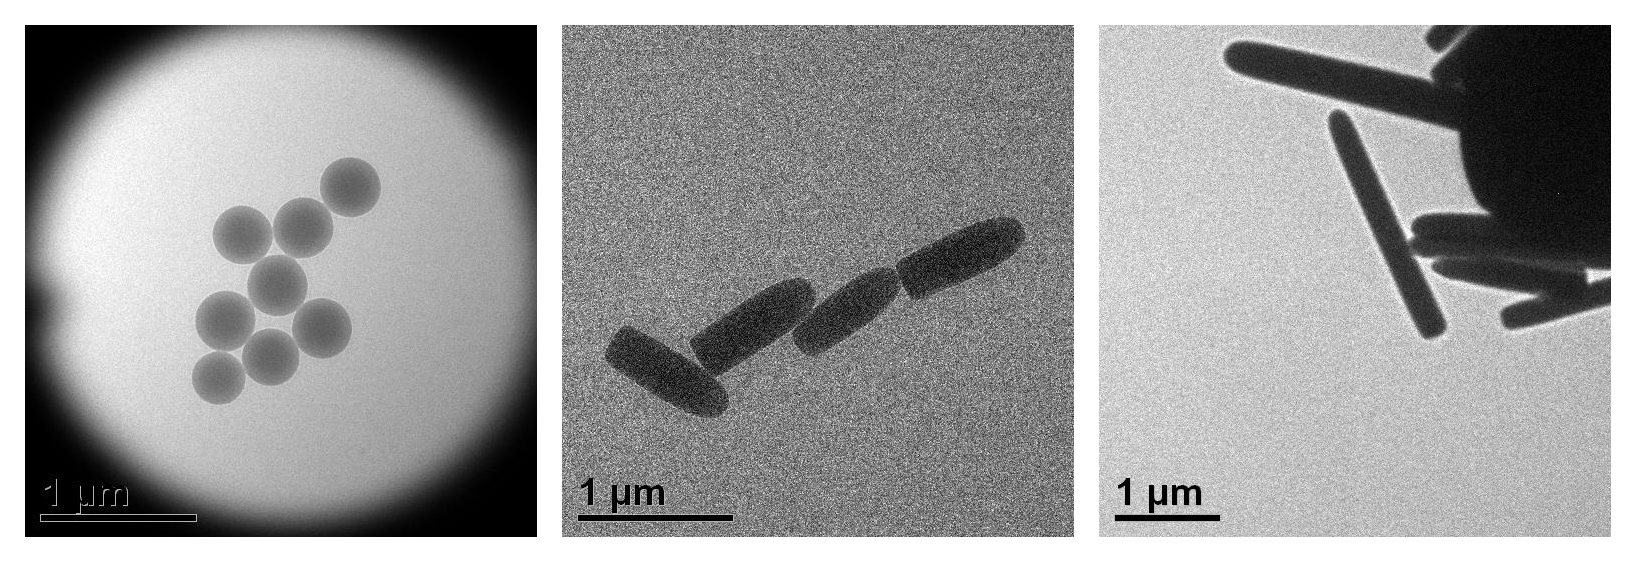
\includegraphics[width=1\textwidth]{particles}
			\caption{\textbf{Transmission electron microscope images of polystyrene beads and silica nanorods.} While the polystyrene beads are nearly perfectly spherical, the silica nanorods are approximately `bullet shaped'. For the purposes of this work, we approximated their shapes as ellipsoids in order to apply equation \ref{eq:dIellipsoid}.}
			\label{fig:particles}
		\end{figure}


	    
		In order to test the principle described above, we performed resistive pulse experiments with single mesopores ranging from $800-\SI{1000}{nm}$ in diameter. The material used was polyethylene terephthalate (PET), a polymer which is known to have highly irregularly shaped interiors when pores are prepared \textit{via} the track-etch technique, as shown in figure \ref{fig:PET}. For the particles, $\SI{410}{nm}$ in diameter polystyrene beads (`spheres') were used as the tracer particle, and rods of length $\SI{590}{nm}$, diameter $\SI{210}{nm}$ (`short rods') and $\SI{1920}{nm}$, diameter $\SI{240}{nm}$ (`long rods') were used to test the length measurement protocol; the particles are shown in figure \ref{fig:particles}. Particles were suspended in $\SI{100}{mM}$ KCl solution with $0.5\%$ Tween 80, a surfactant which prevents particle aggregation. The solution was then injected into both sides of a conductivity cell, and a voltage was applied across the pore. The resulting ionic current was sampled at $\SI{10}{kHz}$ and recorded. The polystyrene spheres used had a larger $\zeta-\mathrm{potential}$ than the pore, and therefore they translocated through the pore electrophoretically. On the other hand, the rods had a lower magnitude $\zeta-\mathrm{potential}$ than the pore, and therefore travelled through the pore under electroosmotic convective forces. 
		
	
	\section{Analysis}
		Events were extracted from the current time series and studied separately.

	
		
		
		
	

	




%%% Local Variables: ***
%%% mode: latex ***
%%% TeX-master: "thesis.tex" ***
%%% End: ***
